\documentclass[a4paper,12pt]{article}
\usepackage[utf8]{inputenc}
\usepackage[T2A]{fontenc}
\usepackage[russian]{babel}
\usepackage{amsmath, amssymb, amsfonts, amsthm}
\usepackage{graphicx}
\usepackage{geometry}
\usepackage{float}
\usepackage[hidelinks, pdfencoding=auto, psdextra]{hyperref}
\usepackage{tocloft}
\usepackage{fancyhdr}
\usepackage{enumitem}
\usepackage{listings}
\usepackage{xcolor}
\usepackage{subcaption}

\geometry{top=2cm, bottom=2cm, left=2cm, right=2cm}
\setlength{\headheight}{14.5pt}

\begin{document}

\begin{titlepage}
    \centering
    {\Large \bfseries Федеральное государственное автономное образовательное учреждение высшего образования «Национальный исследовательский университет ИТМО» \par}
    
    {\large Факультет программной инженерии и компьютерной техники \par}
    \vspace{2cm}
    {\LARGE Домашнее задание №5 \par}
    \vspace{0.5cm}
    {\Large Вариант 74 \par}
    \vspace{2cm}
    \vfill
    \begin{flushright}
        \large
        \textbf{Выполнил:} \\
        Шулай Роман \\
        Группа P3115 \\
        \vspace{1cm}
        \textbf{Преподаватель:} \\
        Поляков Владимир Иванович \\
    \end{flushright}
    \vfill
    {\large Санкт-Петербург \\ 2026 год}
\end{titlepage}
\newpage
\setcounter{page}{2}

\begin{figure}[htbp]
    \centering
    \begin{subfigure}[b]{0.45\textwidth}
        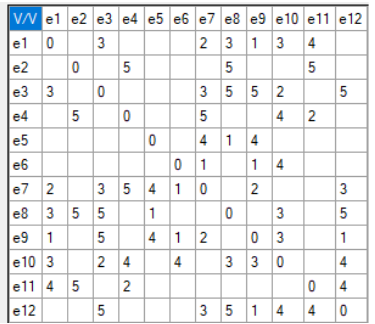
\includegraphics[width=\linewidth]{images/matrix.png}
        \caption{Матрица смежности}
        \label{fig:sub1}
    \end{subfigure}
    \hfill % Распорка для равномерного распределения
    \begin{subfigure}[b]{0.45\textwidth}
        
\includegraphics[width=\linewidth]{images/graph.png}
        \caption{Граф}
        \label{fig:sub2}
    \end{subfigure}
    %\caption{Общая подпись для двух картинок}
    \label{fig:main}
\end{figure}

\noindent 
Исходный граф G1
\begin{table}[H]
    \centering
    \begin{tabular}{|c|c|c|c|c|c|c|c|c|c|c|c|c|c|}
    \hline
        v/v & $e_1$ & $e_2$ & $e_3$ & $e_4$ & $e_5$ & $e_6$ & $e_7$ & $e_8$ & $e_9$ & $e_{10}$ & $e_{11}$ & $e_{12}$ & $p(e)$ \\ \hline
        $e_1$ & 0 & 0 & 1 & 0 & 0 & 0 & 1 & 1 & 1 & 1 & 1 & 0 & 6 \\ \hline
        $e_2$ & 0 & 0 & 0 & 1 & 0 & 0 & 0 & 1 & 0 & 0 & 1 & 0 & 3 \\ \hline
        $e_3$ & 1 & 0 & 0 & 0 & 0 & 0 & 1 & 1 & 1 & 1 & 0 & 1 & 6 \\ \hline
        $e_4$ & 0 & 1 & 0 & 0 & 0 & 0 & 1 & 0 & 0 & 1 & 1 & 0 & 4 \\ \hline
        $e_5$ & 0 & 0 & 0 & 0 & 0 & 0 & 1 & 1 & 1 & 0 & 0 & 0 & 3 \\ \hline
        $e_6$ & 0 & 0 & 0 & 0 & 0 & 0 & 1 & 0 & 1 & 1 & 0 & 0 & 3 \\ \hline
        $e_7$ & 1 & 0 & 1 & 1 & 1 & 1 & 0 & 0 & 1 & 0 & 0 & 1 & 7 \\ \hline
        $e_8$ & 1 & 1 & 1 & 0 & 1 & 0 & 0 & 0 & 0 & 1 & 0 & 1 & 6 \\ \hline
        $e_9$ & 1 & 0 & 1 & 0 & 1 & 1 & 1 & 0 & 0 & 1 & 0 & 1 & 7 \\ \hline
        $e_{10}$ & 1 & 0 & 1 & 1 & 0 & 1 & 0 & 1 & 1 & 0 & 0 & 1 & 7 \\ \hline
        $e_{11}$ & 1 & 1 & 0 & 1 & 0 & 0 & 0 & 0 & 0 & 0 & 0 & 1 & 4 \\ \hline
        $e_{12}$ & 0 & 0 & 1 & 0 & 0 & 0 & 1 & 1 & 1 & 1 & 1 & 0 & 6 \\ \hline
    \end{tabular}
\end{table}

\noindent
Перенумерованный граф G2
\begin{table}[H]
    \centering
    \begin{tabular}{|c|c|c|c|c|c|c|c|c|c|c|c|c|c|}
    \hline
        v/v & $f_1$ & $f_2$ & $f_3$ & $f_4$ & $f_5$ & $f_6$ & $f_7$ & $f_8$ & $f_9$ & $f_{10}$ & $f_{11}$ & $f_{12}$ & $p(f)$ \\ \hline
        $f_1$ & 0 & 1 & 1 & 0 & 0 & 1 & 0 & 1 & 0 & 1 & 0 & 1 & 6 \\ \hline
        $f_2$ & 1 & 0 & 1 & 0 & 0 & 1 & 0 & 1 & 0 & 1 & 1 & 0 & 6 \\ \hline
        $f_3$ & 1 & 1 & 0 & 1 & 0 & 0 & 1 & 1 & 1 & 0 & 1 & 0 & 7 \\ \hline
        $f_4$ & 0 & 0 & 1 & 0 & 1 & 0 & 0 & 0 & 0 & 1 & 0 & 1 & 4 \\ \hline
        $f_5$ & 0 & 0 & 0 & 1 & 0 & 1 & 0 & 0 & 0 & 0 & 0 & 1 & 3 \\ \hline
        $f_6$ & 1 & 1 & 0 & 0 & 1 & 0 & 1 & 0 & 0 & 1 & 1 & 0 & 6 \\ \hline
        $f_7$ & 0 & 0 & 1 & 0 & 0 & 1 & 0 & 1 & 0 & 0 & 0 & 0 & 3 \\ \hline
        $f_8$ & 1 & 1 & 1 & 0 & 0 & 0 & 1 & 0 & 1 & 1 & 1 & 0 & 7 \\ \hline
        $f_9$ & 0 & 0 & 1 & 0 & 0 & 0 & 0 & 1 & 0 & 1 & 0 & 0 & 3 \\ \hline
        $f_{10}$ & 1 & 1 & 0 & 1 & 0 & 1 & 0 & 1 & 1 & 0 & 1 & 0 & 7 \\ \hline
        $f_{11}$ & 0 & 1 & 1 & 0 & 0 & 1 & 0 & 1 & 0 & 1 & 0 & 1 & 6 \\ \hline
        $f_{12}$ & 1 & 0 & 0 & 1 & 1 & 0 & 0 & 0 & 0 & 0 & 1 & 0 & 4 \\ \hline
    \end{tabular}
\end{table}

\noindent
Для графа $G_1$ $\sum p(e) = 62$. Список $P(e) = \{7,7,7,6,6,6,6,4,4,3,3,3\}$ \\
Для графа $G_2$ $\sum p(f) = 62$. Список $P(f) = \{7,7,7,6,6,6,6,4,4,3,3,3\}$ \\

\noindent
Разобьем вершины обоих графов на классы по их степеням
\begin{table}[H]
    \centering
    \begin{tabular}{|c|c|c|c|c|}
    \hline
         & $p(e)=p(f)=7$ & $p(e)=p(f)=6$ & $p(e)=p(f)=4$ & $p(e)=p(f)=3$ \\ \hline
        $E$ & $e_7$, $e_9$, $e_{10}$ & $e_1$, $e_3$, $e_8$, $e_{12}$ & $e_4$, $e_{11}$ & $e_2$, $e_5$, $e_6$ \\ \hline
        $F$ & $f_3$, $f_8$, $f_{10}$ & $f_1$, $f_2$, $f_6$, $f_{11}$ & $f_4$, $f_{12}$ & $f_5$, $f_7$, $f_9$ \\ \hline
    \end{tabular}
\end{table}

\noindent
Рассмотрим сначала класс со степенью $4$. Степени соседей у $e_4$: $3, 4, 7, 7$. А у $e_{11}$: $6,3,4,6$ \\
У $f_4$: $7, 3, 7, 4$, а у $f_{12}$: $6, 4, 3, 6$. Отсюда однозначно $e_4 - f_4$ и $e_{11} - f_{12}$ \\

\noindent
Попробуем связать вершины из класса со степенью $3$ \\
Мы знаем, что у $e_4$ из соседей степени $3$ всего одна вершина: $e_2$. Отсюда однозначно $e_2 - f_5$ (так как $f_5$ - сосед степени $3$ вершины $f_4$) \\
Дальше, у $e_6$ все 3 соседа степени $7$, значит $e_6 - f_9$. Остается, что $e_5 - f_7$ \\

\noindent
Свяжем вершины из класса со степенью $7$ \\
\begin{table}[H]
    \centering
    \begin{tabular}{|c|c|c|c|c|c|c|c|c|c|c|c|c|}
    \hline
        v/v & $e_1$ & $e_2$ & $e_3$ & $e_4$ & $e_5$ & $e_6$ & $e_7$ & $e_8$ & $e_9$ & $e_{10}$ & $e_{11}$ & $e_{12}$ \\ \hline
        $e_2$ & 0 & 0 & 0 & 1 & 0 & 0 & 0 & 1 & 0 & 0 & 1 & 0 \\ \hline
        $e_4$ & 0 & 1 & 0 & 0 & 0 & 0 & 1 & 0 & 0 & 1 & 1 & 0 \\ \hline
        $e_5$ & 0 & 0 & 0 & 0 & 0 & 0 & 1 & 1 & 1 & 0 & 0 & 0 \\ \hline
        $e_6$ & 0 & 0 & 0 & 0 & 0 & 0 & 1 & 0 & 1 & 1 & 0 & 0 \\ \hline
        $e_{11}$ & 1 & 1 & 0 & 1 & 0 & 0 & 0 & 0 & 0 & 0 & 0 & 1 \\ \hline
    \end{tabular}
\end{table}

\begin{table}[H]
    \centering
    \begin{tabular}{|c|c|c|c|c|c|c|c|c|c|c|c|c|}
    \hline
        v/v & $f_1$ & $f_2$ & $f_3$ & $f_4$ & $f_5$ & $f_6$ & $f_7$ & $f_8$ & $f_9$ & $f_{10}$ & $f_{11}$ & $f_{12}$ \\ \hline
        $f_4$ & 0 & 0 & 1 & 0 & 1 & 0 & 0 & 0 & 0 & 1 & 0 & 1 \\ \hline
        $f_5$ & 0 & 0 & 0 & 1 & 0 & 1 & 0 & 0 & 0 & 0 & 0 & 1 \\ \hline
        $f_7$ & 0 & 0 & 1 & 0 & 0 & 1 & 0 & 1 & 0 & 0 & 0 & 0 \\ \hline
        $f_9$ & 0 & 0 & 1 & 0 & 0 & 0 & 0 & 1 & 0 & 1 & 0 & 0 \\ \hline
        $f_{12}$ & 1 & 0 & 0 & 1 & 1 & 0 & 0 & 0 & 0 & 0 & 1 & 0 \\ \hline
    \end{tabular}
\end{table}
\noindent
Анализ вершин показывает соответствия $e_7 - f_3$, $e_9 - f_{10}$ и $e_{10} - f_8$ \\

\noindent
Остается найти соответствия в классе со степенью $6$ \\

\begin{table}[H]
    \centering
    \begin{tabular}{|c|c|c|c|c|c|c|c|c|c|c|c|c|}
    \hline
        v/v & $e_1$ & $e_2$ & $e_3$ & $e_4$ & $e_5$ & $e_6$ & $e_7$ & $e_8$ & $e_9$ & $e_{10}$ & $e_{11}$ & $e_{12}$ \\ \hline
        $e_2$ & 0 & 0 & 0 & 1 & 0 & 0 & 0 & 1 & 0 & 0 & 1 & 0 \\ \hline
        $e_4$ & 0 & 1 & 0 & 0 & 0 & 0 & 1 & 0 & 0 & 1 & 1 & 0 \\ \hline
        $e_5$ & 0 & 0 & 0 & 0 & 0 & 0 & 1 & 1 & 1 & 0 & 0 & 0 \\ \hline
        $e_6$ & 0 & 0 & 0 & 0 & 0 & 0 & 1 & 0 & 1 & 1 & 0 & 0 \\ \hline
        $e_7$ & 1 & 0 & 1 & 1 & 1 & 1 & 0 & 0 & 1 & 0 & 0 & 1 \\ \hline
        $e_9$ & 1 & 0 & 1 & 0 & 1 & 1 & 1 & 0 & 0 & 1 & 0 & 1 \\ \hline
        $e_{10}$ & 1 & 0 & 1 & 1 & 0 & 1 & 0 & 1 & 1 & 0 & 0 & 1 \\ \hline
        $e_{11}$ & 1 & 1 & 0 & 1 & 0 & 0 & 0 & 0 & 0 & 0 & 0 & 1 \\ \hline
    \end{tabular}
\end{table}

\begin{table}[H]
    \centering
    \begin{tabular}{|c|c|c|c|c|c|c|c|c|c|c|c|c|}
    \hline
        v/v & $f_1$ & $f_2$ & $f_3$ & $f_4$ & $f_5$ & $f_6$ & $f_7$ & $f_8$ & $f_9$ & $f_{10}$ & $f_{11}$ & $f_{12}$ \\ \hline
        $f_3$ & 1 & 1 & 0 & 1 & 0 & 0 & 1 & 1 & 1 & 0 & 1 & 0 \\ \hline
        $f_4$ & 0 & 0 & 1 & 0 & 1 & 0 & 0 & 0 & 0 & 1 & 0 & 1 \\ \hline
        $f_5$ & 0 & 0 & 0 & 1 & 0 & 1 & 0 & 0 & 0 & 0 & 0 & 1 \\ \hline
        $f_7$ & 0 & 0 & 1 & 0 & 0 & 1 & 0 & 1 & 0 & 0 & 0 & 0 \\ \hline
        $f_8$ & 1 & 1 & 1 & 0 & 0 & 0 & 1 & 0 & 1 & 1 & 1 & 0 \\ \hline
        $f_9$ & 0 & 0 & 1 & 0 & 0 & 0 & 0 & 1 & 0 & 1 & 0 & 0 \\ \hline
        $f_{10}$ & 1 & 1 & 0 & 1 & 0 & 1 & 0 & 1 & 1 & 0 & 1 & 0 \\ \hline
        $f_{12}$ & 1 & 0 & 0 & 1 & 1 & 0 & 0 & 0 & 0 & 0 & 1 & 0 \\ \hline
    \end{tabular}
\end{table}

\noindent
Анализ вершин показывает соответствия $e_1 - f_1$, $e_3 - f_2$, $e_8 - f_6$ и $e_{12} - f_{11}$ \\

\noindent
Таким образом, каждой вершине графа $G_1$ соответствует вершина из $G_2$ $\Rightarrow$ графы изоморфны

\end{document}